% \documentclass{article}
% \usepackage{graphicx} % Required for inserting images

% \title{ECEN5033_MCS_Proposal}
% \author{razan.alghamdi }
% \date{April 2024}

% \begin{document}

% \maketitle

% \section{Introduction}

% \end{document}


%%%%%%%%%%%%%%%%%%%%%%%%%%%%%%%%%%%%%%%%%%%%%%%%%%%%%%%%%%%%%%%%%%%%%%%%%%%%%%%%
% Template for USENIX papers.
%
% History:
%
% - TEMPLATE for Usenix papers, specifically to meet requirements of
%   USENIX '05. originally a template for producing IEEE-format
%   articles using LaTeX. written by Matthew Ward, CS Department,
%   Worcester Polytechnic Institute. adapted by David Beazley for his
%   excellent SWIG paper in Proceedings, Tcl 96. turned into a
%   smartass generic template by De Clarke, with thanks to both the
%   above pioneers. Use at your own risk. Complaints to /dev/null.
%   Make it two column with no page numbering, default is 10 point.
%
% - Munged by Fred Douglis <douglis@research.att.com> 10/97 to
%   separate the .sty file from the LaTeX source template, so that
%   people can more easily include the .sty file into an existing
%   document. Also changed to more closely follow the style guidelines
%   as represented by the Word sample file.
%
% - Note that since 2010, USENIX does not require endnotes. If you
%   want foot of page notes, don't include the endnotes package in the
%   usepackage command, below.
% - This version uses the latex2e styles, not the very ancient 2.09
%   stuff.
%
% - Updated July 2018: Text block size changed from 6.5" to 7"
%
% - Updated Dec 2018 for ATC'19:
%
%   * Revised text to pass HotCRP's auto-formatting check, with
%     hotcrp.settings.submission_form.body_font_size=10pt, and
%     hotcrp.settings.submission_form.line_height=12pt
%
%   * Switched from \endnote-s to \footnote-s to match Usenix's policy.
%
%   * \section* => \begin{abstract} ... \end{abstract}
%
%   * Make template self-contained in terms of bibtex entires, to allow
%     this file to be compiled. (And changing refs style to 'plain'.)
%
%   * Make template self-contained in terms of figures, to
%     allow this file to be compiled. 
%
%   * Added packages for hyperref, embedding fonts, and improving
%     appearance.
%   
%   * Removed outdated text.
%
%%%%%%%%%%%%%%%%%%%%%%%%%%%%%%%%%%%%%%%%%%%%%%%%%%%%%%%%%%%%%%%%%%%%%%%%%%%%%%%%

\documentclass[letterpaper,twocolumn,10pt]{article}
\usepackage{usenix}

% to be able to draw some self-contained figs
\usepackage{tikz}
\usepackage{amsmath}
\usepackage{tabularx}

% inlined bib file
\usepackage{filecontents}
\usepackage{xspace}

\newcommand{\todo}[1]{\textcolor{red}{{#1}}}

\newcommand{\toolname}{\textit{Leroy}\xspace}

\newcommand{\toolnamepy}{\textit{Leroy4Py}\xspace}

\newcommand{\avgcompression}{1.05x}
% Library Extraction for a Python program

% LEAP

%-------------------------------------------------------------------------------
\begin{filecontents}{\jobname.bib}
%-------------------------------------------------------------------------------
@Book{arpachiDusseau18:osbook,
  author =       {Arpaci-Dusseau, Remzi H. and Arpaci-Dusseau Andrea C.},
  title =        {Operating Systems: Three Easy Pieces},
  publisher =    {Arpaci-Dusseau Books, LLC},
  year =         2015,
  edition =      {1.00},
  note =         {\url{http://pages.cs.wisc.edu/~remzi/OSTEP/}}
}
@InProceedings{waldspurger02,
  author =       {Waldspurger, Carl A.},
  title =        {Memory resource management in {VMware ESX} server},
  booktitle =    {USENIX Symposium on Operating System Design and
                  Implementation (OSDI)},
  year =         2002,
  pages =        {181--194},
  note =         {\url{https://www.usenix.org/legacy/event/osdi02/tech/waldspurger/waldspurger.pdf}}}
\end{filecontents}

%-------------------------------------------------------------------------------
\begin{document}
%-------------------------------------------------------------------------------

%don't want date printed
\date{}

% make title bold and 14 pt font (Latex default is non-bold, 16 pt)
\title{\Large \bf Library Extraction for Imperative Programming Languages}

%for single author (just remove % characters)
\author{
{\rm Abhiram Bellur}\\
CU Boulder
\and
{\rm Razan}\\
CU Boulder
 \and
 {\rm Kudus Workneh}\\
CU Boulder
 \and
{\rm Joseph Izraelevitz}\\
CU Boulder
% \and
% {\rm Joseph Izraelevitz}\\
% CU Boulder
% copy the following lines to add more authors
% \and
% {\rm Name}\\
%Name Institution
} % end author

\maketitle

%-------------------------------------------------------------------------------
\begin{abstract}
%-------------------------------------------------------------------------------
% Library abstraction is the task of learning a library of repetitive or common code functionalities from a given program or set of programs. This compresses code by replacing blocks of code with their appropriate function calls. Library abstraction is also used in program-learning, where an agent learns to write a program from a given corpus of other programs. 

Library learning is the process of building a library of common functionalities from a given set of programs. Typically, this process was applied in the context of aiding program synthesis: concise functions can help the synthesizer build more complex programs. As a result, most library extraction tools 
% like Stitch \cite{Bowers_2023stitch}, 
% This compresses code by replacing blocks of code with their appropriate function calls. 
% Library abstraction is also used in program-learning, where an agent learns to write a program from a given corpus of other programs. 
are designed to abstract over simple domain specific languages (DSL) written in a lisp-like syntax. 

Our work introduces \toolname, which extends library learning techniques to higher level programming languages, while preserving optimality and speed of previous techniques. Our key idea is to leverage a modified version of the program AST which we represent in a lisp-like form to utilise a previous library learning approach. Further, we prune abstractions which cannot be implemented in the programming language and convert the best abstractions back to the original language. 
We implement out technique in a tool for 
% \todo{a subset of} 
the Python programming language, and evaluate it on a multiple corpora of programs. We find an average compression ratio of \avgcompression. Additionally, we show that our technique prunes 
% \todo{75\%} of 
invalid abstractions.

% while checking for semantic equivalence(\todo{90\%}), compression(\todo{150\%}) and usefulness of abstractions (\todo{80\%}).
% This paper introduces \toolname, an extension to Stitch that converts python input to a lisp-like format accepted by the Stitch, then converts the Stitch's output back to python.   
\end{abstract}


%-------------------------------------------------------------------------------
\section{Introduction}
%-------------------------------------------------------------------------------

Software engineers spend a large portion of their time improving the quality of their code. This includes refactoring, improving readability, fixing formatting issues and adding documentation. In particular, engineers often refactor their code bases by abstracting reusable/repeated functionality from their code into library functions. These library functions (also called utility functions) capture parts of the program logic that are used by different software modules. 
Library extraction can be a tedious and error-prone process for developers. 

% While tools that detect code clones and provide extract method suggestions \todo{citation} can be useful to developers, they have a limited vision: only the function to be modified is taken into account. I

Previous work from babble and stitch \cite{Cao_2023babble, Bowers_2023stitch} leverages ideas from dreamcoder \cite{ellis2020dreamcoder} to abstract common functionality from code. However, these tools are aimed at aiding the learning process of program synthesizers. When a program synthesizer learns from a compressed corpus, it is expected to learn writing smaller code that utilizes the abstracted libraries. This reduction of the synthesized output size reduces the errors possibilities. Therefore, prior work focuses abstracting functions for DSLs(domain specific languages) that use a functional lisp-like syntax.  These tools focus generating abstractions that provide the highest compression rate possible.
Ideas from these techniques are unexplored for general purpose programming languages, where developers would also like to abstract common functionality for reusability and maintenance purposes. 
% which lack basic capabilities used by software developers such as conditional statements and loops. 
Library learning is a promising technique, capable of doing two things at once: extracting reusable functions in a recursive manner and rewriting code to find reusable components. 

In this work, we introduce \toolname, a technique that extends library extraction to general purposes programming languages. \toolname performs library extraction by leveraging the AST (abstract syntax tree) of the original program. However, naively abstracting over the AST gives rise to different kinds of invalid abstractions. Abstractions could be macro-like, take in invalid parameters or fail to return necessary variables. We describe these issues in detail in section \todo{3}.  
By modifying existing library extraction techniques, \toolname provides useful and reusable functions that developers can take advantage of. We discover two approaches to present the best abstractions to a user. One, we prune invalid abstractions that are impossible to implement, by checking if each abstraction is a valid and well-formed part of the program's AST. We augment each abstraction with an appropriate return statement.
% \todo{Then, we augment abstractions with the results of a liveness analysis to ensure sensible values are returned.}.
Two, to present the most interesting abstractions to a user, \toolname adds a minimum threshold on the size of the abstraction, to weed out trivial abstractions. 

Our technique lifts library extraction to general-purpose programming languages. We implement our techniques for the the Python programming language in a tool called \toolname.
To evaluate \toolname, we test its compression abilities over a corpora of open source python programs. Additionally, we count the number of invalid abstractions removed by our technique.

% correctness of abstractions along with the compression using a subset of the 150k Python Dataset ~\cite{py150} as further explained in the evaluation section. 

% The rest of the paper is written as follows:
% section blah describes blah
% section blah2 describes blah2


% Again minus results, but including a direction and motivation

%-------------------------------------------------------------------------------
\section{Motivation}
%-------------------------------------------------------------------------------

Stitch~\cite{Bowers_2023stitch} is a State-of-The-Art library abstraction tool that takes in a list of programs written in a lisp-like syntax and outputs a library (a list of abstracted functions) while also re-writing the input programs to utilize the abstracted functions. Stitch uses a Lisp-like syntax because it is designed to operate on Domain Specific Languages (DSLs). Hence, while it works with any simple program that can be written in a lisp-like lambda syntax, it does not generalise well to more complicated programs written in general purpose languages, like python.

% \todo{Add some sentences about why it is interesting to lift stitch to python. Something about how developers would find it useful to have such a tool.}

For example, when Stitch is given a python's abstract Syntax Tree (AST) represented in a lisp style, 
% (tweaked to have a lisp-like lambda format) 
some elements or expressions, like the keywords "while" and "if", or operators like "==" and ">", can be treated as first-class citizens of the programming language. This means that variables could hold such values, or functions could be called with these elements as parameters.
% either variable names or function names depending the lamlispfying implementation.
This is because Stitch is unaware of the programming language it is abstracting over. So, it has no knowledge of what would be a valid abstraction in a language like Python. 
% This can result in incorrect abstractions, like an abstraction that expects "if" or "while" as arguments and treats them as variables. Hence, 
To better generalize Stitch and extend it to a language like Python, we identify and prune such invalid abstractions. \toolname extends Stitch by resolving the follwoing four main issues that arise when naivly passing a lisp-like python AST to Stitch: 

\begin{enumerate}
    \item Trivial Abstractions
    Because stitch optimizes on the abstracted function size relative to its use, it may abstract highly repeated sigle-line functionalities when there are no other larger abstraction candidates. This results in functions that, for example, simple adds two numbers. \toolname eliminates such abstractions by imposing a lower constraint on abstraction size.
    \item Macro-like Abstractions: 
    Stitch treats abstracted libraries as macros. When a functionality is abstracted, it can simply be swapped with a call. This approach impacts program correctness as it results in incomplete abstractions, like abstracting "exp + " from exp+exp. A potential abstraction $add(exp)$ would replace an addition of $1+2$ with the call $add(1) 2$. This is clearly invalid syntax.
    
    \toolname resolves this reconstructing the AST and checking its validity. 
    % To eliminate such abstractions, \toolname reconstructs the python AST from the suggested abstractions, and eliminate suggestions that fail to reconstruct a correct AST.  
    \item Invalid Parameters:
    The search method of stitch treats all tree nodes as potential "holes", or function parameters, which is incorrect in the case of python whose AST nodes are not all first-class citizens. For example, when stitch abstracts over comparative sub-trees, like "x == y" or "x!=z" it can suggest abstractions that takes three parameters, two operands and a comparison operator. A potential abstraction $f(x,op,y)$ would need to be called like: $f(x, ==, y)$ or $f(x, !=, y)$. This is clearly invalid syntax.
    
    \toolname also resolves this reconstructing the AST and checking its validity. 
    \item Incomplete return set:
    Because Stitch treats abstractions as macros, it does not consider variable scoping in abstractions, which impacts code correctness in a language like python. For example, Stitch can abstract assignments without returning the assignment targets. That is, it can suggest functions that change the value of a variable, but never returns the changed variable. In python, such assignment will create a new variable local to the abstracted (called) function instead of changing the value of the variable from the calling function. This, although syntactically correct, changes the program behaviour. This is more advanced issue that is yet to be optimally addressed. Howbeit, \toolname approaches it but attaching a return statement to the abstracted function. \toolname returns the last computed value in the abstraction.
    
\end{enumerate}

% it can be augmented with a python-lisp compiler and a decompiler. The compiler would transform the inputted python programs to the lisp-like format that is passed to Stitch. \toolname then decompiles the output of Stitch back to python. 

%-------------------------------------------------------------------------------
\section{Design }
%-------------------------------------------------------------------------------
% a concrete proposal for how you intend to complete the project


\begin{figure*}
  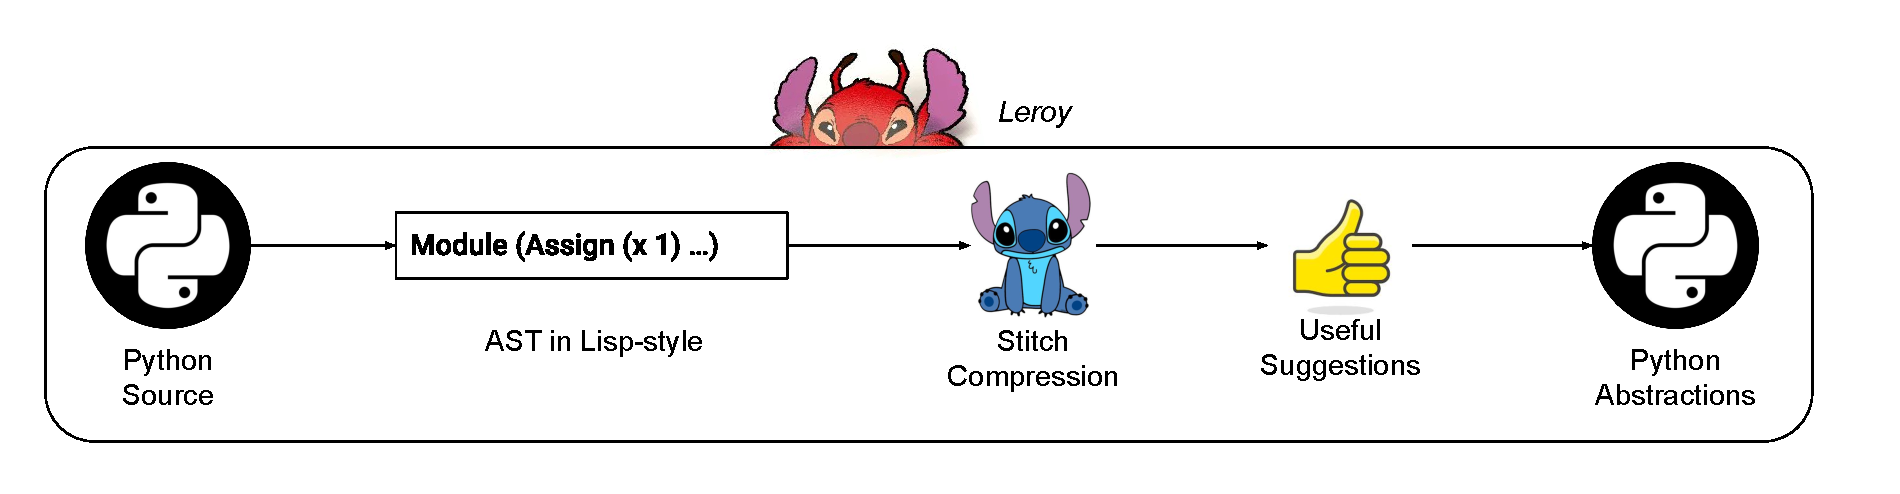
\includegraphics[width=\textwidth]{images/Design.pdf}
  \caption{\toolname's high level design}
  \label{fig:design}
\end{figure*}
\toolname performs library extraction by operating on the AST of the programming language. \toolname uses Stitch \cite{Bowers_2023stitch} as the library extraction engine, prunes invalid abstractions produced by it to present the most useful suggestions to the developer. Figure \ref{fig:design} shows the high level design of \toolname.
% In the sections below, we describe each step in detail.

\subsection{Representing Program AST in a lisp-like form}
To convert program \textbf{ASTs to Lisp}, we treat ASTs as a series of nested function calls, with nodes as the function and subsequent child nodes as the argument of the function. This enables us to unwrap the AST into one long function call.
% \todo{Add diagram of AST and converted lisp?}

\subsection{Pruning Invalid Abstractions}
Stitch suggests abstractions which involve language expressions/statements as function parameters. To \textbf{enhance abstractions} from stitch, we prune such cases. 


\subsubsection{Macro-Like Abstractions}
To prune macro-like abstractions, we attempt to convert the abstraction back into a program AST, and check if the tree is well-formed (all required children of a parent exist). Any incomplete ASTs are deemed to be macro-like and are pruned.

\subsubsection{Invalid Parameters}
We use a similar approach to find cases where invalid parameters could be passed to the abstraction. We convert the abstraction's body into a program AST and encode the abstraction's parameters as identifier nodes. 
Then, we check if these identifier nodes are valid children in the AST. For example, an identifier node cannot be a valid child of a comparison expression's operator. But, an identifier node can be a valid child of the same expression's operand. 

To summarise, if the AST is invalid or not well-formed, we deem the abstraction to be invalid.

\subsection{Presenting Non-trivial Abstractions}

To prune trivial abstractions (e.g. a function which performing addition of two arguments), we introduce a minimum size for the abstraction. This ensures that we have interesting abstractions coming out of \toolname.


\subsection{Figuring out the return value}

We augment the abstraction from Stitch by adding a necessary return value, if it does not exist. Our approach returns the last variable or expression in the abstraction's body. This is a simple approach that ensures that abstractions are functional in the target programming language. 

% We remove abstractions which take language expressions/statements as parameters. 

% \todo{This is the research problem. Add details when we have a more concrete solution.}

% \subsection{Converting Lisp to Language AST}
\subsection{Converting abstractions back to the PL}
Finally, we convert the suggestions from stitch back into the AST. Then, we unparse the AST to result in the compressed code. 

% \todo{add design diagram.}



%-------------------------------------------------------------------------------
\section{Evaluation}
%-------------------------------------------------------------------------------
\section{Evaluation}
\label{sec:eval}


We developed \toolname with Stitch commit number \todo{6fa2...} and we evaluate it on a \todo{xyz} machine running a \todo{xyz} operating system version \todo{xyz}. To evaluate it, we used a corpus of \todo{50} python programs \todo{maybe cite a github link to P2 test cases} that adhere to the P2 grammar described in figure \ref{fig:grammar}. The testing corpus can be found on \todo{github link)} along with \toolname's code. 

Applying Stitch, with no pruning or validation, on lispified input yields \todo{15} total abstracions. Out of which \todo{5} of the \todo{15} found abstractions were trivial, \todo{3} involved macro-like statements, \todo{5} took in invalid parameters and only \todo{2} were valid abstractions. In comparison, applying \toolname to the same input, with the minimum size threshold set to \todo{20} outputs 6 valid abstractions, some of which create and return functions. We found that each abstraction was applied with \todo{3} call sites on average. We compressed the code by \todo{X}.

\todo{what are the other parameters passed in the testing process?}

\todo{rename to methodology? include limitations here? }
% This shows the necessity of our techniques. 

% \toolname is able to find 6 abstractions, after applying our techniques. We used a minimum threshold size of \todo{20} \todo{size unit} to ensure larger sized abstractions. Notably, \toolname was also able to find abstractions that created and returned a function. 





\todo{machine ?}
\todo{Discuss the impact of our pruning methods on utility }
%-------------------------------------------------------------------------------
\section{Related Work}
%-------------------------------------------------------------------------------
% \todo{Section 6, merging all group members drafts, below are the individual drafts}

% Abhiram: 
% \textbf{Program synthesis} aims to auto-generate programs that meet input-output requirements. Most techniques utilise a specialised DSL(domain specific language) to make the synthesis faster and more tractable. 
% Dreamcoder\cite{ellis2020dreamcoder} and EC2 \cite{EC2} lead a line of work\cite{laps, LILO, EC, MCMC} in inductive program synthesis, which takes inspirations from the way humans write code: developing reusable libraries. 
% These techniques take a set of tasks(ex: input, and corresponding outputs), and aim to synthesise programs at meet the task's specifications. To achieve this goal, a two-step process is followed. First, the technique partially synthesises a suite of programs that accomplish the tasks. Then, it learns reusable elements(libraries) from these programs which are further used to enhance the quality of synthesis. 
% % Specifically, DreamCoder uses an EC\textsuperscript{2} (Explore, Compress, Compile) ~\cite{EC2} synthesis algorithm, where it abstracts libraries in one of its 2 sleep stages to explore potential extensions to the given corpus, then compress the found abstractions in the next sleep stage to grow the library used for training the recognition neural network and synthesize programs in the wake stage of the next cycle. However, DreamCoder's success in solving problems in various domains, such as physics laws and text-editing, came with very high time cost. 
% This line of work is designed, or evaluated for learning abstractions over programs written in domain specific languages or lambda calculus. 
% % \todo{It is unclear how these techniques extend to higher-level languages.}
% % LILO uses LLMs to documentation, functional languages.
% % \todo{Add citations to LAPS, LILO, EC2, EC}

% Some works\cite{regal, patios} aim to extend these techniques to high-level languages. PATOIS \cite{patios}, equips and trains a neural synthesizer to use learned code idioms, while Regal\cite{regal} utilises LLMs to synthesise and abstract programs. Both of these techniques do not specifically aim to learn better abstractions.
% % These techniques are primarily 

% \textbf{Learning Abstractions:} 
% % that are useful and repeated in a corpus of programs is the goal of \cite{shapecoder, shapemod, babble, stitch}. 
% Babble\cite{babble} and Stitch\cite{stitch} are two closely related works that focus entirely on library extraction. While babble aims to improve the quality of learned libraries by using e-graphs and rewrite rules, stitch provides guarantees on the size of the learned corpus and the speed at which libraries are learned. 
% ShapeMod\cite{shapemod} and Shapecoder \cite{shapecoder} learn useful and explainable macros by limiting to programs that draw 3D shapes.
% % This line of work is designed, or evaluated for learning abstractions over domain specific languages(such as drawing shapes), or functional programming languages.
% Our work aims to extend these ideas to high-level languages like Python.


% An \textbf{Extract Method refactoring} \cite{jdeo, jextract, gems} aims to extract reusable blocks of code from a function. While these techniques operate on languages commonly used by software developers(Java), most have a limited vision: only the function to be modified is taken into account. In contrast, library learning techniques such a babble\cite{babble} look at the entire corpus of programs as a whole, with the potential to discover abstractions by correctly rewriting programs. 


\subsection{Program synthesis}
Library Abstraction aims to compress code via extracting common functionalities of multiple functions into a single repeatedly used function. However, this is usually done with the bigger goal of generating better libraries to be used for program synthesis (the generation of programs that solve a given problem). Most current state-of-the art work on library extraction are based on DreamCoder ~\cite{ellis2020dreamcoder}, a program synthesizer that adopts the wake-sleep algorithm ~\cite{wake-sleep} to bootstrap inductive program synthesis from a small problem-corpus represented with a Domain Specific Language (DSL). Specifically, DreamCoder uses an EC\textsuperscript{2} (Explore, Compress, Compile) ~\cite{EC2} synthesis algorithm, where it abstracts libraries in one of its 2 sleep stages to explore potential extensions to the given corpus, then compress the found abstractions in the next sleep stage to grow the library used for training the recognition neural network and synthesize programs in the wake stage of the next cycle. However, DreamCoder's success in solving problems in various domains, such as physics laws and text-editing, came with very high time cost. 

\subsection{Library Abstraction}
Subsequent work aimed to enhance DreamCoder via enhancing the abstraction methods. For example, Babble~\cite{Cao_2023babble} proposes utilizing semantics-based abstractions, which results in better abstractions in less time. However, Babble's efficiency comes with an input complexity cost, as in addition to the program corpus, users must also input a semantic equivalence list, which the program uses to abstract common libraries over semantically equivalent programs that look different. Stitch~\cite{Bowers_2023stitch} on the other hand aims to efficiently abstract libraries by reducing the abstraction search space. It does so by defining a utility measure, and performing a top-down search that optimizes utility using the branch and bound method, which eliminates search branches that are upper-bounded by a utility smaller than the current best utility. 

\subsection{Using LLMs}
As discussed earlier, one aim of library abstraction is to enhance program synthesis, which requires the abstracted libraries to be properly documented, which Lilo~\cite{grand2024lilo} covers. To improve program synthesis, lilo utilizes Large Language Models (LLMs) to provide common sense knowledge as a first search step over the string space, before performing an enumerative search over the program space as in DreamCoder. Lilo then uses the Stitch compressor, and once more utilize LLMs to document the resulting libraries with a natural language. The use of the full lilo system enhances performance, in contrast to incorporating LLM guided search without the documentation phase which degrades performance. However, all aforementioned work take in \(lambda\)-calculus and DSL input, unlike ReGAL~\cite{stengeleskin2024regal} which similarly uses LLM-guided search and utilize LLMs in library generation and documentation, but also works with general purpose languages like python. However, ReGAL uses library extraction as a step in program synthesis, where its main goal is to synthesize programs that satisfy a given written task. 

\subsection{Visual Abstraction, Program Learning, and Rewriting}
Other work cover library abstractions with a focus on visual representation programs ~\cite{jones2023shapecoder} ~\cite{wang2021learningVisAbst}~\cite{Jones_2021}. ShapeCoder ~\cite{jones2023shapecoder}  for example uses Neural Networks and e-graphs to not only extract useful abstractions from visual modeling programs, but also explain input shapes using the abstractions. 
Other lines of work, despite not sharing the library extraction focus, share components of programming and natural language processing and recognition. This includes work on program learning~\cite{cropper2019playgol}~\cite{DBLP:journals/corr/abs-2004-09931refproginduc}~\cite{wong2022leveraging}  ~\cite{demo}~\cite{iyer2019learning} ~\cite{hocquette2024learning} and program rewriting~\cite{brandfonbrener2024verified} ~\cite{DBLP:conf/sat/NotzliRBNPBT19rewrite}~\cite{ganeshan2023improving}, which use relevant methods such as finding idioms, and search algorithms as the Monte Carlo tree Search. 




\section{Discussion and Future Work}

\section{Discussion and Future Work}
\label{sec:conc}

Although \toolname generalizes Stitch \cite{Bowers_2023stitch} and addresses 
the main issues Stitch has when fed with python code, it has yet to be more extensively and rigorously tested, 
as well as compared against other previous work. Prior to testing, \toolname can also be extended further to better address 
the stated problems with more advanced program analysis methods, to optimize the current solutions approaches. Furthermore, \toolname extends Stitch without utilising program semantics as babble~\cite{Cao_2023babble} does. Hence, \toolname can be enhanced by adopting from babble and utilizing semantic equivalence to expand the abstraction choices. Lastly, currently \toolname is only tested for compression, but library abstraction for python also targets readability and other program quality metrics that can be encoded in the utility function, and are yet to be tested. 
% \todo{say something about extending from p2 to entire python}



% \begin{enumerate}
%     \item Integration of babble and stitch
%     \item Extension of evaluation
%     \item Comparison against other related work: Regal (novelty), extract-method tools, ast-based code clone detection. Check other work form ICSE/FSE.
%     \item Thoughts about what would make this a full research paper
% \end{enumerate}

% Additionally, \toolname ensures that abstractions involve parameters that are data types.

% Match locations only contain valid function calls.

% Implementation in on ast-completing checking in Rust

% Find a way to measure usefulness/how interesting an abstraction is.
% part of the template
%-------------------------------------------------------------------------------
% \section{Footnotes, Verbatim, and Citations}
% %-------------------------------------------------------------------------------

% Footnotes should be places after punctuation characters, without any
% spaces between said characters and footnotes, like so.%
% \footnote{Remember that USENIX format stopped using endnotes and is
%   now using regular footnotes.} And some embedded literal code may
% look as follows.

% \begin{verbatim}
% int main(int argc, char *argv[]) 
% {
%     return 0;
% }
% \end{verbatim}

% Now we're going to cite somebody. Watch for the cite tag. Here it
% comes. Arpachi-Dusseau and Arpachi-Dusseau co-authored an excellent OS
% book, which is also really funny~\cite{arpachiDusseau18:osbook}, and
% Waldspurger got into the SIGOPS hall-of-fame due to his seminal paper
% about resource management in the ESX hypervisor~\cite{waldspurger02}.

% The tilde character (\~{}) in the tex source means a non-breaking
% space. This way, your reference will always be attached to the word
% that preceded it, instead of going to the next line.

% And the 'cite' package sorts your citations by their numerical order
% of the corresponding references at the end of the paper, ridding you
% from the need to notice that, e.g, ``Waldspurger'' appears after
% ``Arpachi-Dusseau'' when sorting references
% alphabetically~\cite{waldspurger02,arpachiDusseau18:osbook}. 

% It'd be nice and thoughtful of you to include a suitable link in each
% and every bibtex entry that you use in your submission, to allow
% reviewers (and other readers) to easily get to the cited work, as is
% done in all entries found in the References section of this document.

% Now we're going take a look at Section~\ref{sec:figs}, but not before
% observing that refs to sections and citations and such are colored and
% clickable in the PDF because of the packages we've included.

% %-------------------------------------------------------------------------------
% \section{Floating Figures and Lists}
% \label{sec:figs}
% %-------------------------------------------------------------------------------


% %---------------------------
% \begin{figure}
% \begin{center}
% \begin{tikzpicture}
%   \draw[thin,gray!40] (-2,-2) grid (2,2);
%   \draw[<->] (-2,0)--(2,0) node[right]{$x$};
%   \draw[<->] (0,-2)--(0,2) node[above]{$y$};
%   \draw[line width=2pt,blue,-stealth](0,0)--(1,1)
%         node[anchor=south west]{$\boldsymbol{u}$};
%   \draw[line width=2pt,red,-stealth](0,0)--(-1,-1)
%         node[anchor=north east]{$\boldsymbol{-u}$};
% \end{tikzpicture}
% \end{center}
% \caption{\label{fig:vectors} Text size inside figure should be as big as
%   caption's text. Text size inside figure should be as big as
%   caption's text. Text size inside figure should be as big as
%   caption's text. Text size inside figure should be as big as
%   caption's text. Text size inside figure should be as big as
%   caption's text. }
% \end{figure}
% %% %---------------------------


% Here's a typical reference to a floating figure:
% Figure~\ref{fig:vectors}. Floats should usually be placed where latex
% wants then. Figure\ref{fig:vectors} is centered, and has a caption
% that instructs you to make sure that the size of the text within the
% figures that you use is as big as (or bigger than) the size of the
% text in the caption of the figures. Please do. Really.

% In our case, we've explicitly drawn the figure inlined in latex, to
% allow this tex file to cleanly compile. But usually, your figures will
% reside in some file.pdf, and you'd include them in your document
% with, say, \textbackslash{}includegraphics.

% Lists are sometimes quite handy. If you want to itemize things, feel
% free:

% \begin{description}
  
% \item[fread] a function that reads from a \texttt{stream} into the
%   array \texttt{ptr} at most \texttt{nobj} objects of size
%   \texttt{size}, returning returns the number of objects read.

% \item[Fred] a person's name, e.g., there once was a dude named Fred
%   who separated usenix.sty from this file to allow for easy
%   inclusion.
% \end{description}

% \noindent
% The noindent at the start of this paragraph in its tex version makes
% it clear that it's a continuation of the preceding paragraph, as
% opposed to a new paragraph in its own right.


% \subsection{LaTeX-ing Your TeX File}
% %-----------------------------------

% People often use \texttt{pdflatex} these days for creating pdf-s from
% tex files via the shell. And \texttt{bibtex}, of course. Works for us.

% %-------------------------------------------------------------------------------
% \section*{Acknowledgments}
% %-------------------------------------------------------------------------------

% The USENIX latex style is old and very tired, which is why
% there's no \textbackslash{}acks command for you to use when
% acknowledging. Sorry.

% %-------------------------------------------------------------------------------
% \section*{Availability}
% %-------------------------------------------------------------------------------

% USENIX program committees give extra points to submissions that are
% backed by artifacts that are publicly available. If you made your code
% or data available, it's worth mentioning this fact in a dedicated
% section.

%-------------------------------------------------------------------------------
\bibliographystyle{plain}
\bibliography{references}
% \bibliography{\jobname}

%%%%%%%%%%%%%%%%%%%%%%%%%%%%%%%%%%%%%%%%%%%%%%%%%%%%%%%%%%%%%%%%%%%%%%%%%%%%%%%%
\end{document}
%%%%%%%%%%%%%%%%%%%%%%%%%%%%%%%%%%%%%%%%%%%%%%%%%%%%%%%%%%%%%%%%%%%%%%%%%%%%%%%%

%%  LocalWords:  endnotes includegraphics fread ptr nobj noindent
%%  LocalWords:  pdflatex acks